\begin{tcolorbox}[colback=gray!5,colframe=gray!80,title=\textbf{Scheda Informativa}]
\begin{itemize}
    \item \textbf{Luogo}:  \emph{Quantum Measurement}
    \item \textbf{Giorno e ora}: Il tempo non è osservabile
    \item \textbf{Situazione}: Laura e Marley stanno fuggendo.
\end{itemize}
\end{tcolorbox}

\vspace{1em}
\begin{center}Laura\end{center}
\hrule
\vspace{1em}

 Marley e io fuggivamo attraverso gli stretti corridoi. L'eco metallico dei nostri passi si avvicinava alla frequenza del mio cuore. Improvvisamente, una serie di urla strazianti squarciò il silenzio. Era un suono agghiacciante, simile a un coro di disperazione proveniente da un'altra dimensione. Mi fermai di colpo, il cuore mi martellava nel petto.

\begin{dialogue}
\speak{Laura} \enquote{Cosa sta succedendo?} chiesi, cercando di mantenere la calma nonostante il terrore che mi pervadeva.

\speak{Marley} \enquote{È il suono dei qubit che collassano} rispose Marley, il volto pallido e teso. \enquote{Stanno subendo le conseguenze del processo di misura. Non riescono a mantenere il loro stato, e quando questo accade... l'effetto è devastante.}
\end{dialogue}

Una stretta gelida mi avvolse lo stomaco. Quelle urla sembravano avere il potere di destabilizzare anche i qubit più stabili.

\begin{dialogue}
\speak{Laura} \enquote{E Caterina?} domandai, la voce incrinata dall'angoscia. \enquote{Dove si trova adesso?}

\speak{Marley}  \enquote{Se non è già stata portata nel \textit{Faulty Qubit Space}, è probabile che sia ancora nel \textit{Fault Tolerance Coding}. Ma dobbiamo muoverci in fretta, dal FQS non potremo più salvarla.}

\speak{Laura} \enquote{Agiamo subito!} esclamai, sentendo l'urgenza crescere dentro di me.

\speak{Marley} Prese un respiro profondo. \enquote{La verità è che, per trovare Caterina, dovremmo prima sconfiggere il Commissario. È sicuramente sua prigioniera.}

\speak{Laura} Feci un passo indietro, incredula. \enquote{Sconfiggere il Commissario? Ma chi è il Commissario?}

\speak{Marley} \enquote{Un traditore. Vuole costruire un sistema parallelo per spodestare il \textit{Quantum Master Program}} rispose. \enquote{\'E l'unico modo. Se vogliamo salvare Caterina e gli altri, dobbiamo agire.}
\end{dialogue}

Mentre cercavamo un nascondiglio tra le ombre del \textit{Quantum Measurement}, un suono metallico e ronzante ci fece sobbalzare. Dai corridoi oscuri alle nostre spalle, due droni \textit{CH4} comparvero, fluttuando come presenze spettrali. Ciascun drone, con i suoi quattro rotori disposti a tetraedro, emetteva una luce soffusa che si rifletteva sulle pareti, mentre due figure scure erano in sella: gli agenti della \textit{Quantum Control Electronics}, inviati per trovarci.

Ci accovacciammo dietro una serie di circuiti e componenti, trattenendo il fiato. I due agenti atterrarono con precisione e, scendendo dai droni, iniziarono a perlustrare l'area. I loro volti erano inespressivi, ma gli occhi scrutavano attentamente ogni dettaglio,  non andavano a caso e ci avrebbero scoperto.  Non avevamo molto tempo. Dovevamo agire in fretta, o saremmo state scoperte.

Marley mi lanciò uno sguardo, cercando una direzione sicura, ma l'intero spazio sembrava chiuso, senza vie di fuga evidenti. Restammo in attesa, pronte a muoverci al primo segnale, sperando di riuscire a eludere gli agenti e sfuggire alla sorveglianza della \textit{Quantum Control Electronics}.

\section{I due agenti}
\vspace{1em}
\begin{center}PzIA\end{center}
\hrule
\vspace{1em}
Gli agenti si muovono con movimenti misurati, esaminando l'area circostante. Uno dei due abbassa la voce e si rivolge al compagno.

\begin{quote}
\enquote{Pensi che possano essersi nascoste nel settore di stabilizzazione dei qubit? Quel posto è praticamente un labirinto,} sussurra, lanciando uno sguardo preoccupato ai droni in standby accanto a loro.
\end{quote}

Il secondo agente mantiene lo sguardo fisso su ogni angolo e su ogni ombra.

\begin{quote}
\enquote{Possibile. Ma se sono abbastanza furbe, potrebbero aver scelto un luogo meno ovvio} risponde.
\end{quote}

Il primo agente annuisce, mostrando segni di tensione.

\begin{quote}
\enquote{Meglio non fare errori. Sai cosa è successo all'ultima squadra che ha fallito una missione sotto gli occhi del Supervisore...}
\end{quote}

Il secondo agente interrompe, con un leggero brivido.

\begin{quote}
\enquote{Non ricordarmelo. Il Supervisore non perdona. E peggio ancora, c'è il \textit{Quantum Master Program} che supervisiona tutto. Nessuna deroga alla coerenza, nessuna possibilità di sfuggire alle direttive.}
\end{quote}

Entrambi gli agenti rivolgono uno sguardo ai droni, gioelli della nanotecnologia sotto la loro diretta responsabilità. Abbandonarli era sempre un rischio. Dopo un momento di silenzio, il secondo agente riprende con voce più ferma.

\begin{quote}
\enquote{Concentriamoci. Dobbiamo trovarle prima che la situazione sfugga di mano. Altrimenti saremo noi a pagarne le conseguenze.}
\end{quote}

Il primo agente annuisce nuovamente, prendendo un respiro profondo.

\begin{quote}
\enquote{Sì, hai ragione. Controlliamo quest'area con attenzione. E speriamo che siano più vulnerabili di quanto ci aspettiamo.}
\end{quote}

\section{La Fuga sul Drone CH4}
\vspace{1em}
\begin{center}Laura\end{center}
\hrule
\vspace{1em}

 Il cuore mi si appesantiva al pensiero del rischio imminente. Eppure, dentro di me, qualcosa si stava risvegliando.

\begin{dialogue}
\speak{Laura} \enquote{Potremmo fuggire con uno di quei droni \textit{CH4}. Potremmo saltarci sopra e raggiungere il \textit{Fault Tolerance Coding} prima che sia troppo tardi!}
\end{dialogue}

Marley scosse la testa, il viso cupo.

\begin{dialogue}
\speak{Marley} \enquote{Non è così semplice. Abbiamo provato a usarli, ma non ci siamo mai riusciti. I droni sono dotati di sistemi di sicurezza e le probabilità di farci scoprire sono alte. Inoltre il passaggio da qui verso il \textit{Fault Tolerance Coding} è sorvegliato da un filtro molecolare, non potremmo mai superarlo a bordo di un $CH_4$.}
\speak{Laura} \enquote{Possiamo andare a piedi?}
\speak{Marley} \enquote{Fuori discussione....}
\speak{Laura} \enquote{Esiste un'alternativa?}
\speak{Marley} \enquote{Possiamo passare per la CCU, se riusciamo a superarla proseguire verso la \textit{Quantum Control Electronics}  e quindi rientrare nel QA. Da li esiste un accesso non controllato verso il \textit{Fault Tolerance Coding}, ma...}
\speak{Laura} \enquote{Ma cosa? C'è qualche problema?}
\speak{Laura} \enquote{Niente. Meglio affrontare i problemi quando si pongono di fronte} concluse. Non aggiunsi altro. 
\end{dialogue}

Guardai il drone \textit{CH4}, un oggetto affascinante e al contempo intimidatorio.

\begin{dialogue}
\speak{Laura} \enquote{Dobbiamo provare, non vedo alternative} dissi indicando il drone.
\end{dialogue}

\begin{dialogue}
\speak{Marley} Marley cercò di mantenere il tono calmo, ma parlò senza mai prendere fiato: \enquote{Laura, ascolta. Non è solo questione di scappare. Dobbiamo avere un piano. Quel drone non ci porterà lontano se non abbiamo il controllo. Non possiamo permettere che i nostri sforzi siano vani.}
\end{dialogue}



%---from here

%--- to here

Strinsi i denti e scrutai il drone: qualcosa doveva pur esserci. Un'idea si faceva largo tra il caos.

\begin{dialogue}
\speak{Laura} \enquote{Aspetta... quel drone, ha la geometria di una molecola di metano. Se è davvero così, allora ha spin totale 1. Forse possiamo controllarlo modificando la proiezione dello spin lungo l'asse Z.}
\end{dialogue}

Marley mi guardò, gli occhi spalancati.

Forse arrossii.

\begin{dialogue}
\speak{Laura} \enquote{Ho solo... ho studiato queste cose. Ho messo insieme qualche indizio. Forse mi sbaglio...}
\end{dialogue}

Marley iniziò a sospettare che non fossi del tutto come lei. E io? Io cominciavo a sospettare che forse... non fossi nemmeno più del tutto nel mio mondo.


\begin{dialogue}
\speak{Marley} \enquote{Sei una \textit{Quantum Crafter}, vero?}
\end{dialogue}

Arrossii leggermente.

\begin{dialogue}
\speak{Laura} \enquote{Non è il momento di parlarne. Dobbiamo agire ora!}
\end{dialogue}

\begin{center}
\begin{minipage}{0.7\textwidth}
    \centering
    \fbox{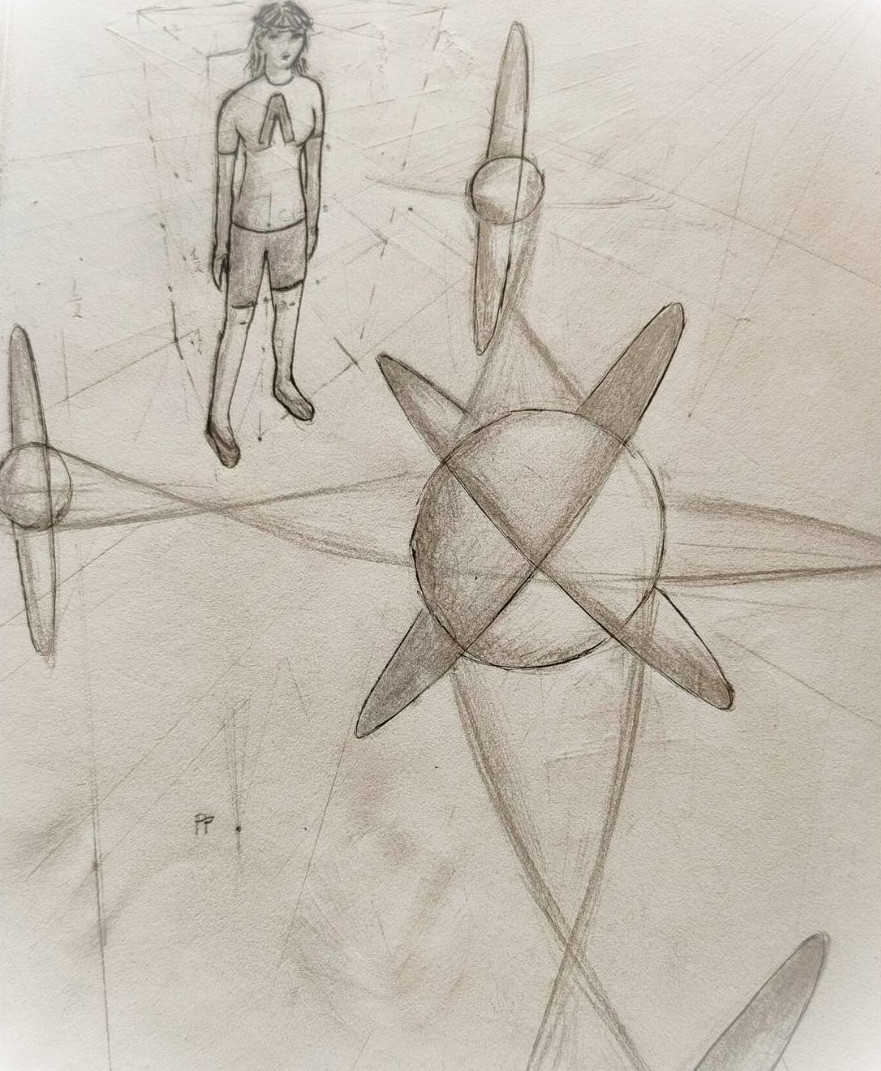
\includegraphics[width=\textwidth]{immagini/cnot_50.jpeg}} % Sostituisci con il nome del file immagine
\end{minipage}
\end{center}

\section{Il Piano di Fuga}

\begin{dialogue}
\speak{Laura} \enquote{Quello sembra un sistema a spin totale 1. Probabilmente si manovra modificando la proiezione dello spin lungo l’asse Z. Dobbiamo provarci!}
\end{dialogue}

Per un attimo mi vidi dall'esterno, sospesa tra paura e coraggio. Mi osservavo da fuori di me. Negli occhi brillava la determinazione. Volevo affrontare il mio destino.


Marley, pur impressionata dalla mia sicurezza, sembrava esitante.

\begin{dialogue}
\speak{Marley} \enquote{Laura, aspetta! Non abbiamo idea di come farlo funzionare. Potrebbe essere troppo pericoloso!}
\end{dialogue}

Ma non potevo permettermi di esitare. Ogni istante di inattività poteva significare la perdita definitiva di Caterina. Mi avvicinai al drone con il cuore che batteva forte per la paura, ma anche per il richiamo dell'azione.

Mi lanciai sull'agente più vicino, che cadde a terra, colto di sorpresa. Senza esitazione, saltai verso il drone, ma ovviamente non me l'avrebbe regalata così facilmente. Mi afferrò per una caviglia facendomi rovinare a terra spinta dal mio stesso impulso. Il drone era ad un soffio dovevo solo liberarmi da quella stretta prima che arrivasse anche l'altro. Sentii un urlo alle mie spalle, qualcosa o qualcuno lo aveva colpito. Ma certo, Marley! Aveva trovato la forza e mi aveva aiutata. Saltammo  sul drone.  Afferrai i comandi orbitali. Il carbonio era freddo, gli atomi di idrogeno tesi al limite: non era il massimo, ma poteva andare. Non era il mio scooter, ma potevamo farcela!




\begin{center}
\begin{minipage}{0.7\textwidth}
    \centering
    \fbox{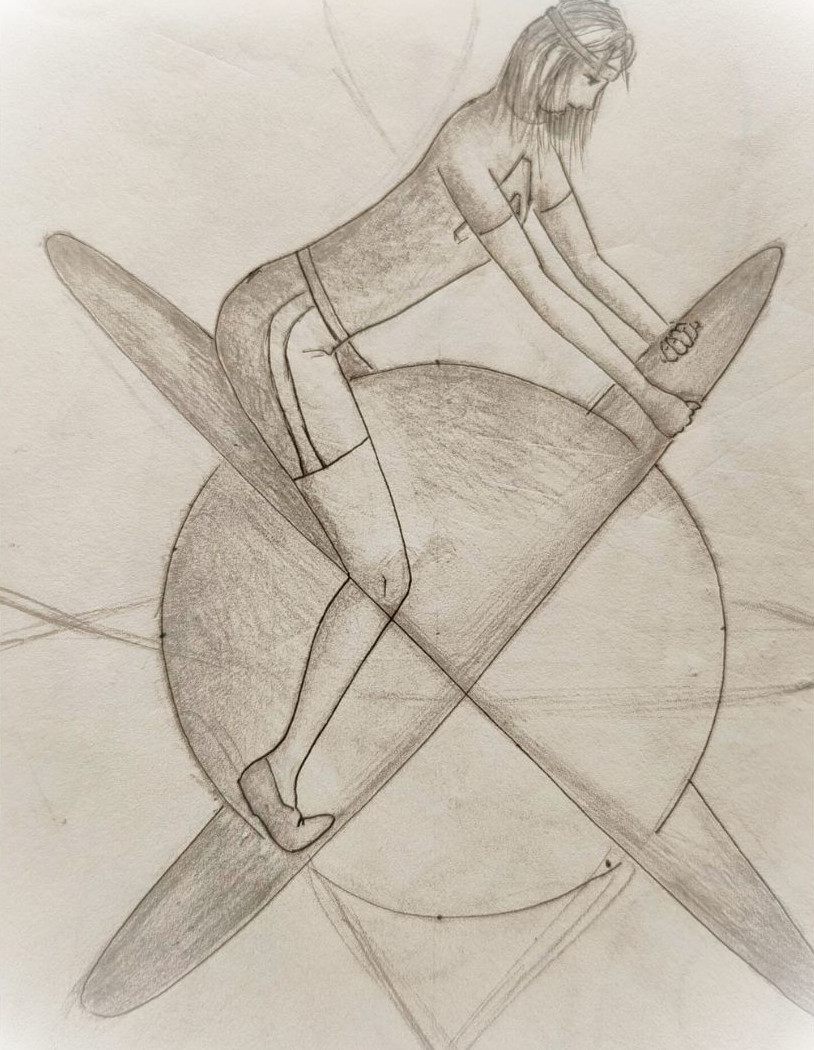
\includegraphics[width=\textwidth]{immagini/cnot_51.jpeg}} % Sostituisci con il nome del file immagine
\end{minipage}
\end{center}


\begin{dialogue}
\speak{Laura} \enquote{Non possiamo fallire. Insieme, possiamo farcela!}
\end{dialogue}

Marley annuì, e le paure che l'avevano trattenuta iniziarono a svanire.

\begin{dialogue}
\speak{Marley} \enquote{D'accordo, Laura. Facciamo in modo che funzioni. Se siamo rapide, possiamo arrivare al \textit{Fault Tolerance Coding} prima che trasferiscano Caterina!}
\end{dialogue}

Con il cuore in gola e la determinazione che pulsava come un'onda di energia, attivai il drone. La superficie  brillava mentre gli oribitali iniziavano a girare, emettendo un sibilo potente che vibrava nell'aria circostante. L'adrenalina scorreva potente, e mentre il drone si sollevava da terra, una nuova speranza si accese dentro di me. Eravamo pronte a lanciarci verso l'ignoto, verso il salvataggio della nostra amica.

\begin{dialogue}
\speak{Marley} \enquote{Vai ora, dirigiti verso quel condensatore, lì c'è il passaggio per la CCU.} In quel momento sentii l'energia che provavo quando da bambina mio padre mi leggeva Salgari. ``Andiamo, papà'' pensai, mentre il suo ricordo mi sfiorò per un istante.
\end{dialogue}
